
% $Header: /cvsroot/latex-beamer/latex-beamer/solutions/generic-talks/generic-ornate-15min-45min.en.tex,v 1.5 2007/01/28 20:48:23 tantau Exp $

\documentclass[smaller]{beamer}
\mode<presentation>
{
  \usetheme{Singapore}
  \usefonttheme[onlymath]{serif}
  % or ...
 %  \setbeamercovered{transparent}
  % or whatever (possibly just delete it)
}


\usepackage[czech]{babel}
% or whatever
\usepackage[utf8]{inputenc}
\usepackage{multicol}
% or whatever
%\usepackage{times}
%\usepackage[T1]{fontenc}
% Or whatever. Note that the encoding and the font should match. If T1
% does not look nice, try deleting the line with the fontenc.


\title{PAS14 -- Tests of independence of random variables}

\author{Jan B\v rezina}
\institute % (optional, but mostly needed)
{
  %\inst{2}%
  Technical University of Liberec
}


% If you wish to uncover everything in a step-wise fashion, uncomment
% the following command: 

%\beamerdefaultoverlayspecification{<+->}

% ***************************************** SYMBOLS
\def\div{{\rm div}}
\def\Lapl{\Delta}
\def\grad{\nabla}
\def\supp{{\rm supp}}
\def\dist{{\rm dist}}
%\def\chset{\mathbbm{1}}
\def\chset{1}

\def\Tr{{\rm Tr}}
\def\sgn{{\rm sgn}}
\def\to{\rightarrow}
\def\weakto{\rightharpoonup}
\def\imbed{\hookrightarrow}
\def\cimbed{\subset\subset}
\def\range{{\mathcal R}}
\def\leprox{\lesssim}
\def\argdot{{\hspace{0.18em}\cdot\hspace{0.18em}}}
\def\Distr{{\mathcal D}}
\def\calK{{\mathcal K}}
\def\FromTo{|\rightarrow}
\def\convol{\star}
\def\impl{\Rightarrow}
\DeclareMathOperator*{\esslim}{esslim}
\DeclareMathOperator*{\esssup}{ess\,sup}
\DeclareMathOperator{\ess}{ess}
\DeclareMathOperator{\osc}{osc}
\DeclareMathOperator{\curl}{curl}

%\def\Ess{{\rm ess}}
%\def\Exp{{\rm exp}}
%\def\Implies{\Longrightarrow}
%\def\Equiv{\Longleftrightarrow}
% ****************************************** GENERAL MATH NOTATION
\def\Real{{\rm\bf R}}
\def\Rd{{{\rm\bf R}^{\rm 3}}}
\def\RN{{{\rm\bf R}^N}}
\def\D{{\mathbb D}}
\def\Nnum{{\mathbb N}}
\def\Measures{{\mathcal M}}
\def\d{\,{\rm d}}               % differential
\def\sdodt{\genfrac{}{}{}{1}{\rm d}{{\rm d}t}}
\def\dodt{\genfrac{}{}{}{}{\rm d}{{\rm d}t}}

\def\vc#1{\mathbf{\boldsymbol{#1}}}     % vector
\def\tn#1{{\mathbb{#1}}}    % tensor
\def\abs#1{\lvert#1\rvert}
\def\Abs#1{\bigl\lvert#1\bigr\rvert}
\def\bigabs#1{\bigl\lvert#1\bigr\rvert}
\def\Bigabs#1{\Big\lvert#1\Big\rvert}
\def\ABS#1{\left\lvert#1\right\rvert}
\def\norm#1{\bigl\Vert#1\bigr\Vert} %norm
\def\close#1{\overline{#1}}
\def\inter#1{#1^\circ}
\def\ol#1{\overline{#1}}
\def\ul#1{\underline{#1}}
\def\eqdef{\mathrel{\mathop:}=}     % defining equivalence
\def\where{\,|\,}                    % "where" separator in set's defs
\def\timeD#1{\dot{\overline{{#1}}}}

% ******************************************* USEFULL MACROS
\def\RomanEnum{\renewcommand{\labelenumi}{\rm (\roman{enumi})}}   % enumerate by roman numbers
\def\rf#1{(\ref{#1})}                                             % ref. shortcut
\def\prtl{\partial}                                        % partial deriv.
\def\Names#1{{\scshape #1}}
\def\rem#1{{\parskip=0cm\par!! {\sl\small #1} !!}}

\def\Xint#1{\mathchoice
{\XXint\displaystyle\textstyle{#1}}%
{\XXint\textstyle\scriptstyle{#1}}%
{\XXint\scriptstyle\scriptscriptstyle{#1}}%
{\XXint\scriptscriptstyle\scriptscriptstyle{#1}}%
\!\int}
\def\XXint#1#2#3{{\setbox0=\hbox{$#1{#2#3}{\int}$}
\vcenter{\hbox{$#2#3$}}\kern-.5\wd0}}
\def\ddashint{\Xint=}
\def\dashint{\Xint-}

% ******************************************* DOCUMENT NOTATIONS
% document specific
\def\rh{\varrho}
\def\vl{{\vc{u}}}
\def\th{\vartheta}
\def\vx{\vc{x}}
\def\vX{\vc{X}}
\def\vr{\vc{r}}
\def\veta{\vc{\eta}}
\def\dx{\,\d\vx}
\def\dt{\,\d t}
\def\bulk{\zeta}
\def\cS{\close{S}}
\def\eps{\varepsilon}
\def\phi{\varphi}
\def\Bog{{\mathcal B}}
\def\Riesz{{\mathcal R}}
\def\distr{\mathcal D}
\def\Item{$\bullet$}

\def\MEtst{\mathcal T}
%***************************************************************************
\setbeamercolor{my blue}{fg=blue}
\def\blue#1{{\usebeamercolor[fg]{my blue} #1}}

\setbeamercolor{my green}{fg=green}
\def\green#1{{\usebeamercolor[fg]{my green} #1}}

% color for term definition
\setbeamercolor{my orange}{fg=orange}
\def\df#1{{\usebeamercolor[fg]{my orange} #1}}
\def\xskip{{\vspace{2ex}}}

\def\cz#1{{\small (#1)}}

\def\E{\vc{\mathsf{E}}}

\begin{document}

\begin{frame}
  \titlepage
\end{frame}

\begin{frame}{Motivation problem}
Do people choose a person with similer height as a partner or not? 

\xskip
Contingency table (cross table):
\begin{center}
\begin{tabular}{r|rrr|r}
 & man-tall & man-medium & man-short & total\\
\hline 
woman-tall & 18 & 20 & 12 & 50\\
woman-medium & 28 & 51 & 25 & 104\\
woman-short & 14 & 28 & 9 & 51\\
\hline
total & 60 & 99 & 46 & 205
\end{tabular}
\end{center}

source [Yule]
\end{frame}


\begin{frame}{Notation}
Consider random vector $\vc X= (Y, Z)$ with discrete distribution, where
$Y\in 1,\dots,r$ and $Z\in1,\dots,c$. We denote:
\[
 p_{ij}=P(Y=i,Z=j),\qquad p_{i.}=\sum_j p_{ij},\qquad p_{.j}=\sum_i p_{ij}
\]

\xskip
For a selection from the distribution $\vc X$ of size $n$, we have random variables $n_{ij}$ - the frequency,
with \blue{multinomial distribution}. These forms \df{contingency table}. We denote:
\[
   n_{i.}=\sum_j n_{ij},\qquad n_{.j}=\sum_i p_{ij},\qquad n=\sum_{i,j} p_{ij}
\]
\dots \df{marginal frequencies}

\end{frame}

\begin{frame}{Independence of variables}
\begin{theorem}
Discrete variables $Y$ and $Z$ are independent if and only if $p_{ij}=p_{i.}p_{.j}$.
\end{theorem}

\xskip
\blue{Proof:}
The independece of variables $Y$ and $Z$: 
\[
  P(Y\in A, Z\in B)=P(Y\in A)P(Z\in B).
\]

From this we have:
\[
  p_{ij}=P(Y\in \{i\}, Z\in \{j\}) = P(Y\in \{i\}) P(Z\in \{j\}) = p_{i.}p_{.j}. 
\]

Oposite implication (we assume $p_{ij}=p_{i.}p_{.j}$):\\
\[
 P(Y\in A, Z\in B)= \sum_{i\in A} \sum_{j\in B} p_{ij} = \sum_{i\in A} p_{i.} \sum_{j\in B} p_{.j} = P(Y\in A)P(Z\in B)
\]

\end{frame}

\begin{frame}{Independence hypothesis}
We want to test hypothesis $H_0$ about independence of $Y$ and $Z$, which is same as:
\[
  H_0: p_{ij}=p_{i.}p_{.j}
\]
Thus probabilities $p_{ij}$ of multinomial distribution depends on $r+c-2$ parameters,
marginal probabilities save $p_{r.}$ and $p_{.c}$ which are given by condition:
\[
   \sum_i p_{i.} = \sum_j p_{.j} = 1
\]
Minimizing 
\[
  \chi^2 = \sum_i \sum_j \frac{ (n_{ij} - np_{ij})^2 }{np_{ij}}
\]
we get best estimates
\[
   \hat{p}_{i.} = \frac{n_{i.}}{n}, \qquad \hat{p}_{.j}=\frac{n_{.j}}{n}
\]

\end{frame}

\begin{frame}{Chi square test of independence}
Test statistics
\[
  \chi^2 = \sum_i \sum_j \frac{ (n_{ij} - m_{ij})^2 }{m_{ij}}, \text{where } m_{ij}=\frac{n_{i.}n_{.j}}{n}
\]
has under hypothesis $H_0$ approximately $\chi^2$ distribution  with 
\[
   rc-(r+c-2)-1 =  (r-1)(c-1)
\]
degrees of freedom.

\xskip
Assumptions:
\begin{itemize}
 \item Random sample, independent samples
 \item 5 observations in every cell (small tables)\\
 or in 80\% of cells (large tables)
\end{itemize}

\end{frame}

\begin{frame}{Example}
\[
  n=205,\quad df=4
\]

\begin{multicols}{2}
\[n_{ij} - m_{ij}\] 
\begin{tabular}{r|rrr}
 & mT & mM & mS \\
\hline 
wT & 3.36 & -4.14 &  0.78 \\
wM & -2.43 & 0.77 & 1.66 \\
wS & -0.92 & 3.37 & -2.44 
\end{tabular}

\[(n_{ij} - m_{ij})^2/m_{ij}\]
\begin{tabular}{r|rrr}
 & mT & mM & mS \\
\hline 
  wT &0.77 &0.71 &0.05\\
  wM &0.20 &0.01 &0.12\\
  wS &0.06 &0.46 &0.52
\end{tabular}
\end{multicols}
\[
    T=2.9,\quad p_{val}=1-F_{\chi^2,4}(T)=0.57
\]
\end{frame}




\begin{frame}[fragile]{R : convert data frame to table}
\begin{verbatim}
> df=read.table("14_tab.dat")
> df
  freq w m
1   18 T T
2   20 T M
3   12 T S
4   28 M T
5   51 M M
6   25 M S
7   14 S T
8   28 S M
9    9 S S
> tab=xtabs(freq~w + m, data=df) 
> tab
   m
w    M  S  T
  M 51 25 28
  S 28  9 14
  T 20 12 18
\end{verbatim}
\end{frame}


\begin{frame}[fragile]{R: test}
\begin{verbatim}
> chisq.test(tab)

        Pearson's Chi-squared test

data:  tab
X-squared = 2.9072, df = 4, p-value = 0.5735

> fisher.test(tab)

        Fisher's Exact Test for Count Data

data:  tab
p-value = 0.5803
alternative hypothesis: two.sided
\end{verbatim}
\end{frame}

\begin{frame}[fragile]{Mosaic plot}
\hbox{
    \kern-5ex\vbox{
        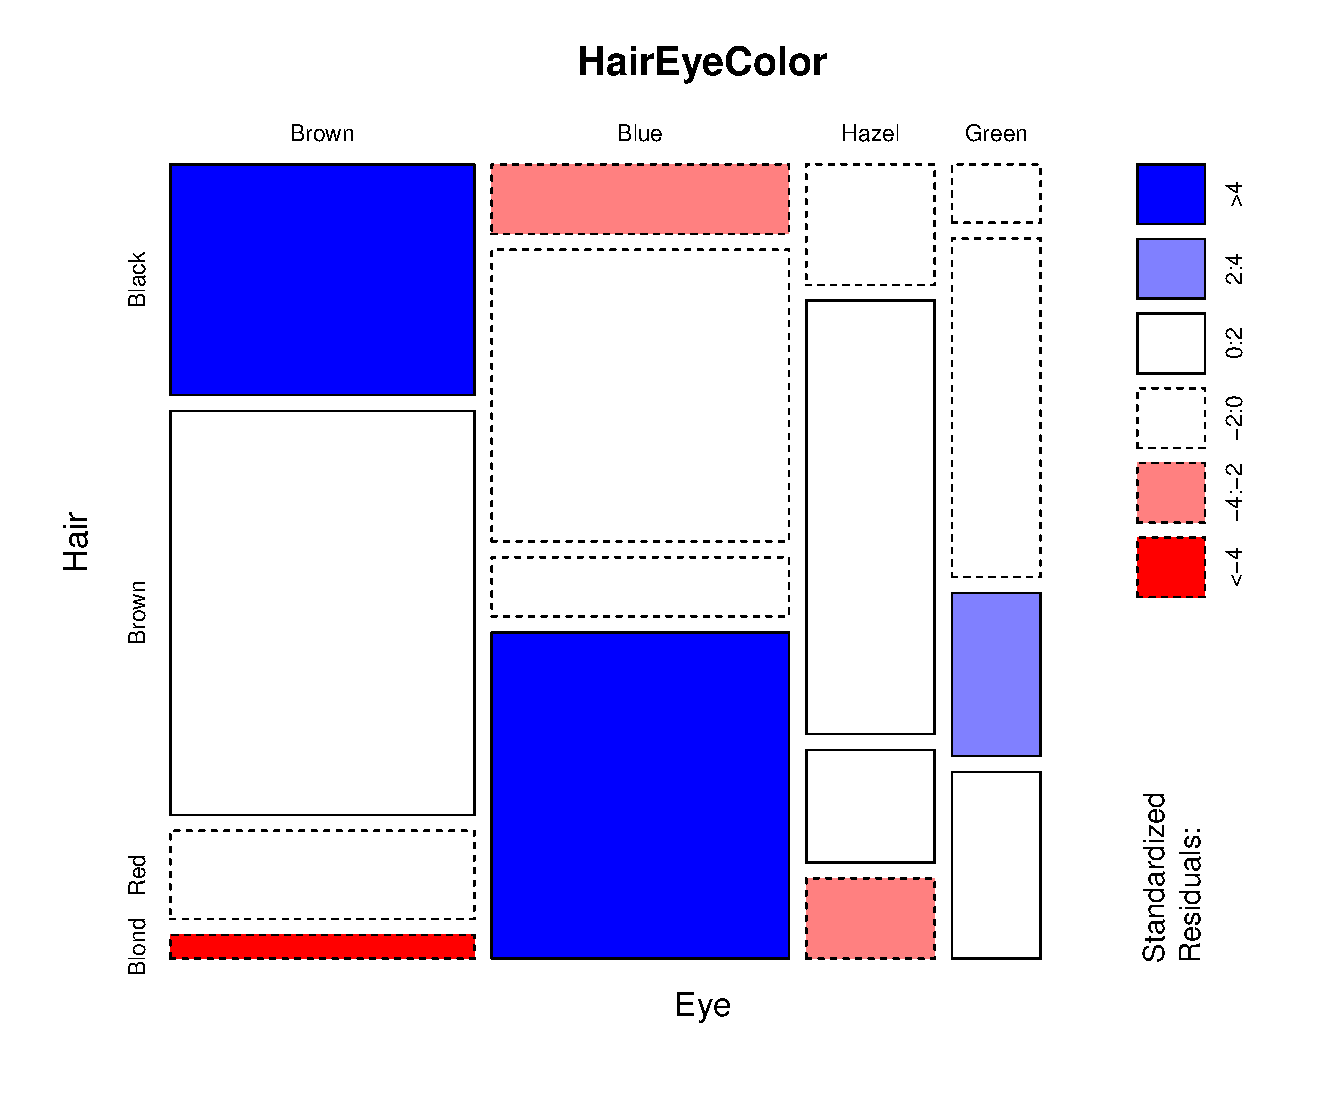
\includegraphics[scale=0.3]{14_Eye_Hair.pdf}\\
        {\tiny \verb'mosaicplot(~Eye+Hair,data=HairEyeColor, shade=T)'}
    }
    \kern-27ex\vbox{
        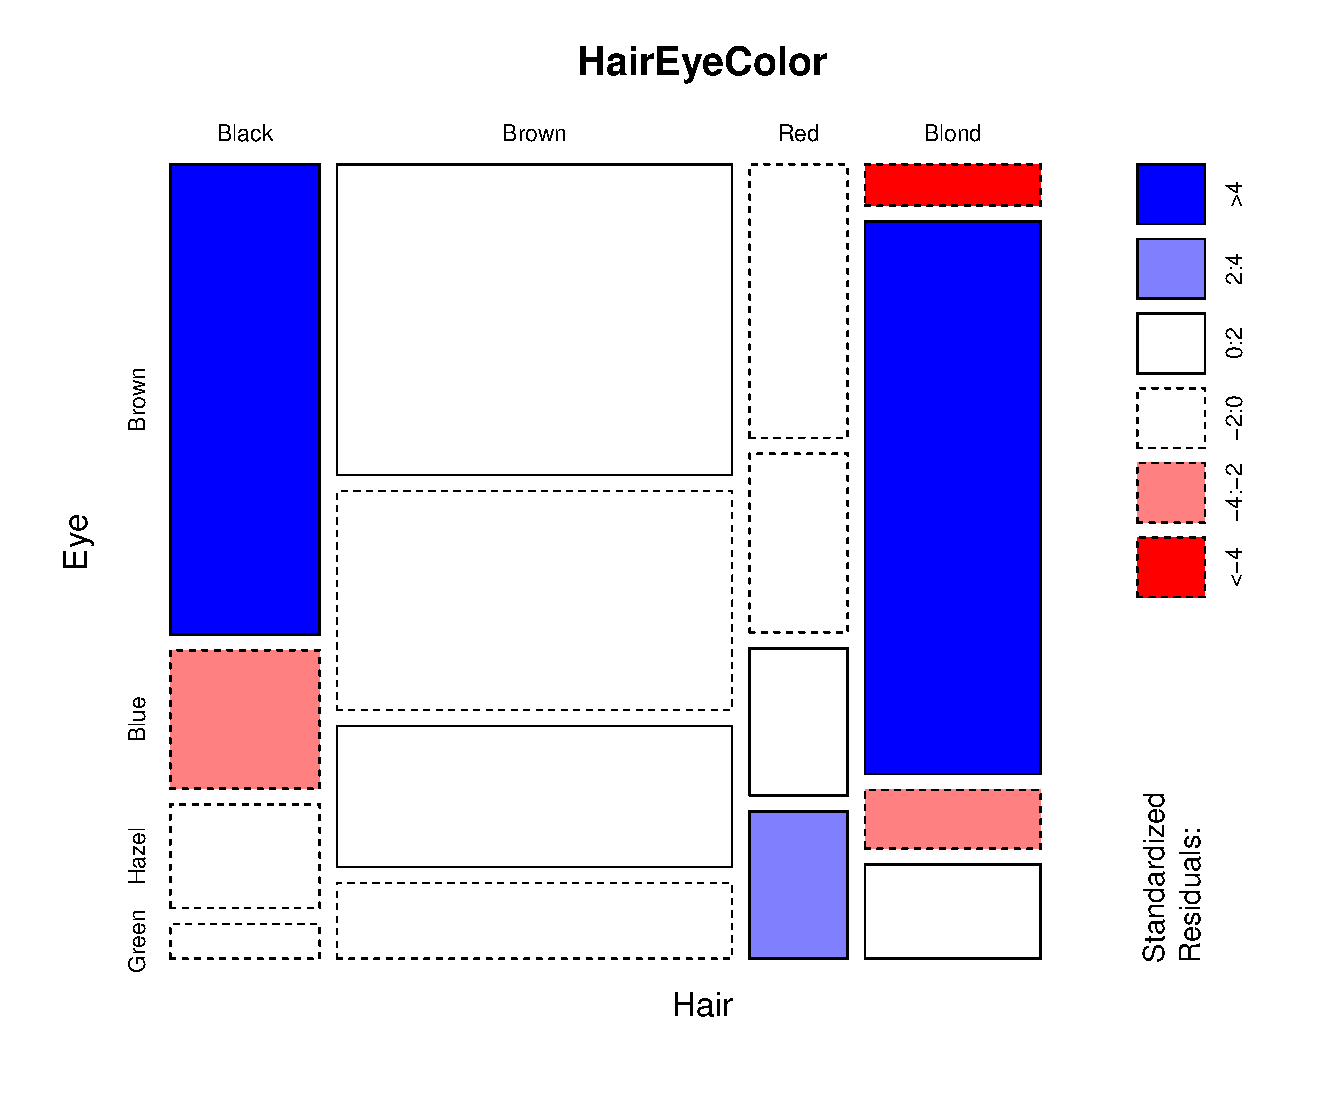
\includegraphics[scale=0.3]{14_Hair_Eye.pdf}\\
        {\tiny \verb'mosaicplot(~Hair+Eye,data=HairEyeColor, shade=T)'}
    }
}    
\end{frame}

\begin{frame}{Extensions}
\begin{itemize}
 \item 3-way tables and interactions
 \item post-hoc analysis
\end{itemize}
 
\end{frame}


\end{document}


